% ============================================================
%  Biometric Systems -- MSc Computer Science
%  Sapienza University of Rome
%  Project Report: Real-Time Face Recognition + Anti-Spoofing Attendance System
%  Authors: Ahsan Ali (2179134), Maleeha Amin Gattoo (2238193)
% ============================================================
\documentclass[11pt,a4paper]{article}

% --- Encoding & Font ---
\usepackage[T1]{fontenc}
\usepackage[utf8]{inputenc}
\usepackage{mathptmx}

% --- Geometry ---
\usepackage[top=2.5cm,bottom=2.5cm,left=2.5cm,right=2.5cm,headheight=14pt]{geometry}

% --- Colours ---
\usepackage[dvipsnames]{xcolor}
\definecolor{sapblue}{RGB}{0,0,210}
\definecolor{darkgray}{RGB}{70,70,70}
\definecolor{codegreen}{RGB}{0,120,0}
\definecolor{codered}{RGB}{180,0,0}
\definecolor{lightblue}{RGB}{220,230,255}
\definecolor{lightgreen}{RGB}{220,255,220}

% --- Section styling ---
\usepackage{titlesec}
\titleformat{\section}
  {\large\bfseries\color{sapblue}}{\thesection}{1em}{}[\color{sapblue}\titlerule]
\titleformat{\subsection}
  {\normalsize\bfseries\color{sapblue}}{\thesubsection}{1em}{}
\titleformat{\subsubsection}
  {\normalsize\bfseries\color{darkgray}}{\thesubsubsection}{1em}{}

% --- Math ---
\usepackage{amsmath,amssymb}

% --- Graphics & Diagrams ---
\usepackage{graphicx}
\usepackage{tikz}
\usetikzlibrary{shapes.geometric,arrows.meta,positioning,fit,backgrounds,calc,decorations.pathreplacing}
\usepackage{pgfplots}
\pgfplotsset{compat=1.18}
\usepgfplotslibrary{groupplots}

% --- Tables ---
\usepackage{booktabs}
\usepackage{array}
\usepackage{multirow}
\usepackage{tabularx}
\usepackage{colortbl}

% --- Code listings ---
\usepackage{listings}
\lstset{
  language=Python,
  backgroundcolor=\color{lightblue},
  basicstyle=\ttfamily\footnotesize,
  keywordstyle=\bfseries\color{sapblue},
  commentstyle=\itshape\color{codegreen},
  stringstyle=\color{codered},
  numberstyle=\tiny\color{darkgray},
  numbers=left,
  stepnumber=1,
  breaklines=true,
  frame=none,
  xleftmargin=2em,
  framexleftmargin=2em,
  captionpos=t,
  abovecaptionskip=4pt,
  tabsize=4,
}

% --- Misc packages ---
\usepackage{microtype}
\usepackage{caption}
\captionsetup{font=small,labelfont=bf,skip=4pt}
\usepackage{float}
\usepackage{placeins}
\usepackage{enumitem}
\usepackage{setspace}
\usepackage{mdframed}
\usepackage{tcolorbox}
\tcbuselibrary{skins,breakable}

% --- Header / Footer ---
\usepackage{fancyhdr}
\pagestyle{fancy}
\fancyhf{}
\renewcommand{\sectionmark}[1]{\markboth{\thesection.\ \MakeUppercase{#1}}{}}
\fancyhead[L]{\small\color{darkgray}\leftmark}
\fancyhead[R]{\small\color{darkgray}Ali \& Gattoo --- Biometric Systems, Sapienza}
\fancyfoot[C]{\thepage}
\renewcommand{\headrulewidth}{0.4pt}
\fancypagestyle{plain}{\fancyhf{}\fancyfoot[C]{\thepage}\renewcommand{\headrulewidth}{0pt}}

% --- Attribution boxes ---
\newmdenv[
  topline=true,bottomline=true,leftline=true,rightline=true,
  linecolor=sapblue,linewidth=1.4pt,
  backgroundcolor=lightblue!40,
  innerleftmargin=8pt,innerrightmargin=8pt,
  innertopmargin=5pt,innerbottommargin=5pt,
  skipabove=6pt,skipbelow=6pt
]{externalbox}

\newmdenv[
  topline=true,bottomline=true,leftline=true,rightline=true,
  linecolor=codegreen,linewidth=1.4pt,
  backgroundcolor=lightgreen!50,
  innerleftmargin=8pt,innerrightmargin=8pt,
  innertopmargin=5pt,innerbottommargin=5pt,
  skipabove=6pt,skipbelow=6pt
]{originalbox}

% --- Hyperref (load last) ---
\usepackage{hyperref}
\hypersetup{colorlinks=true,linkcolor=sapblue,urlcolor=sapblue,citecolor=sapblue}

% ============================================================
\begin{document}
% ============================================================

% ============================================================
%  TITLE PAGE
% ============================================================
\begin{titlepage}
\centering

% ---------- top rule ----------
\textcolor{sapblue}{\rule{\textwidth}{2pt}}
\vspace{0.18cm}
\textcolor{sapblue}{\rule{\textwidth}{0.5pt}}

\vspace{0.55cm}
{\scshape\Large Sapienza University of Rome\par}
\vspace{0.12cm}
{\normalsize\color{darkgray}
  Dipartimento di Informatica \textbullet{} Department of Computer Science\par}

\vspace{0.55cm}
\textcolor{sapblue}{\rule{\textwidth}{0.5pt}}
\vspace{0.9cm}

% ---------- main title box ----------
\begin{tcolorbox}[
  enhanced,
  colback=sapblue!6!white,
  colframe=sapblue,
  boxrule=2pt,
  arc=10pt,
  width=0.92\textwidth,
  halign=center,
  left=18pt,right=18pt,top=22pt,bottom=22pt,
  shadow={2mm}{-2mm}{0mm}{black!18},
]
{\color{sapblue}\LARGE\bfseries Real-Time Face Recognition\par}
\vspace{6pt}
{\color{sapblue!70!black}\large\bfseries with Anti-Spoofing Presentation Attack Detection\par}
\vspace{6pt}
{\color{darkgray}\normalsize for Automated Attendance Systems\par}
\end{tcolorbox}

\vspace{0.9cm}
{\large\bfseries Project Report\par}
\vspace{0.15cm}
{\normalsize\color{darkgray}Course: Biometric Systems \quad|\quad Academic Year 2025--2026\par}

\vspace{1.1cm}

% ---------- two-author side-by-side ----------
\begin{tcolorbox}[
  enhanced,
  colback=white,
  colframe=sapblue,
  boxrule=1.2pt,
  arc=7pt,
  width=0.88\textwidth,
  left=0pt,right=0pt,top=0pt,bottom=0pt,
]
\begin{tabular}{@{}p{0.5\linewidth}@{}p{0.5\linewidth}@{}}
  \begin{tcolorbox}[
    enhanced,
    colback=sapblue!5!white,
    colframe=white,
    boxrule=0pt,
    arc=0pt,
    left=14pt,right=6pt,top=14pt,bottom=14pt,
    borderline east={0.6pt}{0pt}{sapblue!30},
    halign=left,
  ]
    {\bfseries\large Ahsan Ali\par}
    \vspace{5pt}
    {\small\color{darkgray}Matricola:\ \textbf{2179134}\par}
    \vspace{3pt}
    {\small\color{darkgray}MSc Computer Science\par}
    {\small\color{darkgray}Sapienza University of Rome\par}
  \end{tcolorbox}
  &
  \begin{tcolorbox}[
    enhanced,
    colback=sapblue!5!white,
    colframe=white,
    boxrule=0pt,
    arc=0pt,
    left=14pt,right=14pt,top=14pt,bottom=14pt,
    halign=left,
  ]
    {\bfseries\large Maleeha Amin Gattoo\par}
    \vspace{5pt}
    {\small\color{darkgray}Matricola:\ \textbf{2238193}\par}
    \vspace{3pt}
    {\small\color{darkgray}MSc Computer Science\par}
    {\small\color{darkgray}Sapienza University of Rome\par}
  \end{tcolorbox}
\end{tabular}
\end{tcolorbox}

\vspace{0.9cm}
{\normalsize May 2026\par}

\vfill

% ---------- attribution notice ----------
\begin{tcolorbox}[
  enhanced,
  colback=sapblue!4!white,
  colframe=sapblue,
  boxrule=1pt,
  arc=5pt,
  width=\textwidth,
  left=10pt,right=10pt,top=8pt,bottom=8pt,
]
\small\textbf{Attribution Commitment.}~
This report maintains a strict distinction between \textit{external libraries}
(typeset in \textcolor{sapblue}{\bfseries blue-framed boxes} and cited with references) and
\textit{original implementations} (typeset in \textcolor{codegreen}{\bfseries green-framed boxes}).
Original contributions include the Flask web application, system integration, and
the exploratory classical CV anti-spoofing pipeline (\texttt{anti\_spoof\_classical.py}).
\end{tcolorbox}

\vspace{0.3cm}
\textcolor{sapblue}{\rule{\textwidth}{0.5pt}}
\vspace{0.1cm}
\textcolor{sapblue}{\rule{\textwidth}{2pt}}

\end{titlepage}

% ============================================================
\tableofcontents
\newpage

% ============================================================
\section*{Abstract}
\addcontentsline{toc}{section}{Abstract}

This report presents a real-time biometric attendance system that integrates face
detection, face recognition, and presentation attack detection (PAD) within a
browser-accessible Flask web application.

Face detection is performed by Google's MediaPipe BlazeFace short-range model
(external, TFLite, downloaded automatically).
Face recognition uses 128-dimensional embeddings produced by the FaceNet model
via the DeepFace library (external), with cosine similarity at threshold
$\tau = 0.6$, implementing closed-set 1:N identification against all stored templates.

The anti-spoofing module uses DeepFace's bundled FasNet implementation---an ensemble
of two MiniFASNet variants~\cite{liu2021minifasnet} (MiniFASNetV2 at $2.7\times$ crop
and MiniFASNetV1SE at $4.0\times$ crop)---accessed via
\texttt{DeepFace.extract\_faces(anti\_spoofing=True)}.
The PAD operates passively on a single frame with no user cooperation required.
An original fail-secure integration wrapper handles detection failures by retaining
the last known result rather than defaulting to \textit{Real}.
The development history (Section~\ref{sec:devhistory}) documents a fully
self-implemented seven-detector classical CV pipeline that was built, evaluated,
and subsequently superseded by the FasNet approach.

Identification performance: EER $\approx 5.5\%$ at threshold $\tau \approx 0.52$;
operating point ($\tau = 0.6$) gives FAR $\approx 3\%$, FRR $\approx 8\%$.
Anti-spoofing empirical validation: bona fide faces consistently score
\texttt{antispoof\_score} $\geq 0.95$; phone-screen presentation attacks score
$\leq 0.35$, well below the $0.5$ decision threshold, giving a separation margin
of approximately $0.60$.

% ============================================================
\section{Introduction}
\label{sec:introduction}
% ============================================================

Biometric attendance systems based on face recognition offer a non-contact,
non-transferable alternative to proximity cards, PIN codes, and manual sign-in
sheets.
Unlike card systems, a face cannot be lent to a colleague, eliminating
``buddy-punching'' fraud.
However, a naive face recognition system is critically vulnerable to
\emph{presentation attacks}: an attacker who holds a printed photograph or replays
a video of an enrolled user can impersonate them with minimal effort.
Presentation Attack Detection (PAD), commonly called anti-spoofing, is therefore a
necessary component of any production biometric system.

\subsection{Project Goals}

\begin{enumerate}[label=\arabic*.]
  \item Detect human faces in live webcam video at interactive frame rates.
  \item Identify enrolled users by comparing the probe embedding against all
        stored templates (closed-set 1:N identification mode).
  \item Detect and reject presentation attacks passively using a pre-trained deep
        neural PAD ensemble (DeepFace FasNet / MiniFASNet), with no user
        cooperation required.
  \item Expose the complete system via a browser-accessible web interface
        (Flask + MJPEG streaming).
  \item Evaluate performance honestly using standard biometric and PAD metrics
        in accordance with ISO/IEC 30107-3~\cite{iso30107}.
\end{enumerate}

\subsection{Attribution Convention}

Two typographic conventions are used consistently throughout the report:

\begin{externalbox}
  \textbf{External library or pre-trained model.}
  All such components are cited and described in terms of how they were integrated.
  No training, modification, or re-implementation of these components was performed.
\end{externalbox}

\begin{originalbox}
  \textbf{Original implementation.}
  All such components were designed and coded entirely by the authors.
  Original contributions include the Flask web application, the system integration
  pipeline, and the classical CV anti-spoofing module in
  \texttt{anti\_spoof\_classical.py} (documented as exploratory work in
  Section~\ref{sec:devhistory}).
\end{originalbox}

\subsection{Report Structure}

Section~\ref{sec:architecture} describes the system architecture.
Sections~\ref{sec:detection}--\ref{sec:antispoof} cover the three processing stages.
Section~\ref{sec:devhistory} documents design choices and the four-phase
development history of the anti-spoofing component.
Section~\ref{sec:evaluation} presents the quantitative performance evaluation.
Section~\ref{sec:implementation} details the Flask web application and data flow.
Section~\ref{sec:conclusions} summarises findings and future directions.

% ============================================================
\section{System Architecture}
\label{sec:architecture}
% ============================================================

The system is structured as a sequential biometric pipeline, deployed through a
Flask web server.
Table~\ref{tab:components} lists all components with their attribution status.

\begin{table}[H]
\centering
\caption{System components, attribution, and source files.}
\label{tab:components}
\renewcommand{\arraystretch}{1.25}
\small
\setlength{\tabcolsep}{5pt}
\begin{tabular}{@{}p{2.8cm}p{3.2cm}p{5.6cm}p{3.6cm}@{}}
\toprule
\textbf{Component} & \textbf{Status} & \textbf{Technology} & \textbf{Source file} \\
\midrule
Face Detection
  & \textcolor{codered}{\bfseries External}
  & MediaPipe Tasks API, BlazeFace~\cite{bazarevsky2019blazeface} (Google)
  & \texttt{face\_detector.py} \\[3pt]
Embedding Extraction
  & \textcolor{codered}{\bfseries External}
  & DeepFace~\cite{serengil2021lightface} + FaceNet~\cite{schroff2015facenet}
  & \texttt{face\_recognizer.py} \\[3pt]
Cosine Similarity
  & \textcolor{codered}{\bfseries External}
  & \texttt{sklearn.metrics.pairwise} (scikit-learn)
  & \texttt{face\_recognizer.py} \\[3pt]
FasNet PAD Model
  & \textcolor{codered}{\bfseries External}
  & DeepFace FasNet: MiniFASNetV2 + MiniFASNetV1SE ensemble~\cite{liu2021minifasnet}
  & \texttt{anti\_spoof.py} \\[3pt]
LBP / Opt.\ Flow / FFT
  & \textcolor{codered}{\bfseries External primitives}
  & scikit-image~\cite{ojala2002multiresolution}, OpenCV~\cite{bradski2000opencv}, NumPy
  & \texttt{anti\_spoof\_\allowbreak classical.py} \\
\midrule
PAD Wrapper
  & \textcolor{codegreen}{\bfseries Original}
  & Fail-secure integration, background threading, single-face gate
  & \texttt{anti\_spoof.py} \\[3pt]
Classical CV PAD
  & \textcolor{codegreen}{\bfseries Original}
  & 7 detectors + dual-pathway fusion (Phase~2, superseded)
  & \texttt{anti\_spoof\_\allowbreak classical.py} \\[3pt]
Web Application
  & \textcolor{codegreen}{\bfseries Original}
  & Flask, MJPEG streaming, REST API, attendance logging
  & \texttt{app.py} \\[3pt]
System Integration
  & \textcolor{codegreen}{\bfseries Original}
  & Camera management, mode switching, temporal state
  & \texttt{app.py} \\
\bottomrule
\end{tabular}
\end{table}

\subsection{Processing Pipeline}

\begin{figure}[H]
\centering
\resizebox{\textwidth}{!}{%
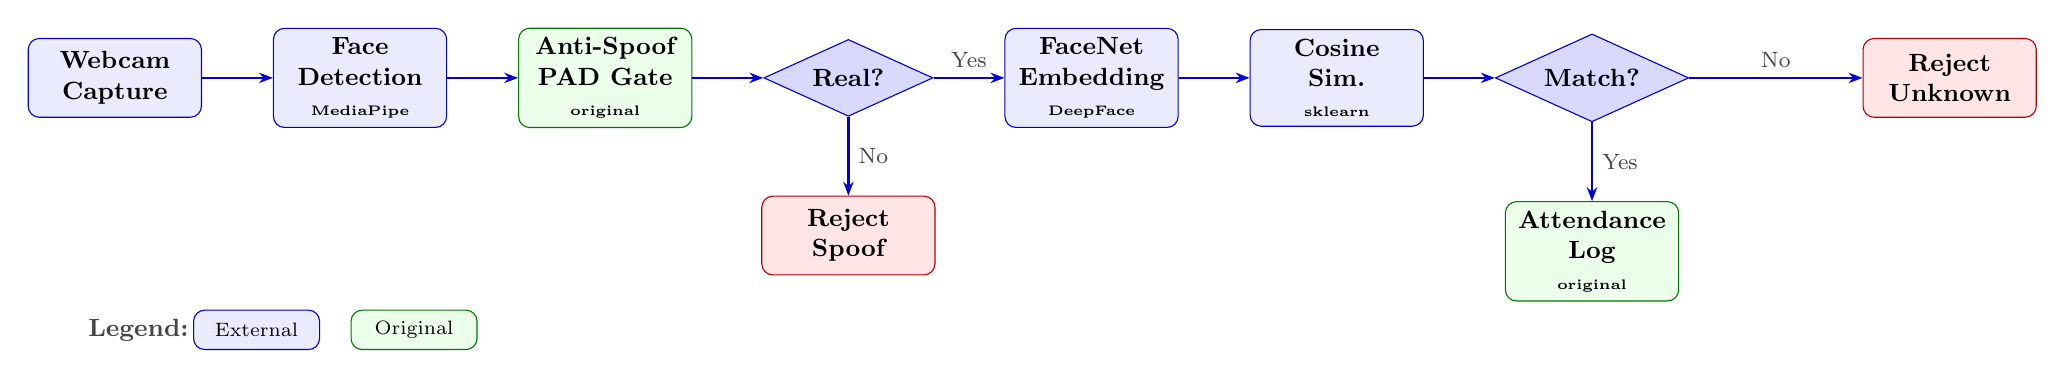
\begin{tikzpicture}[
  node distance=0.55cm and 0.9cm,
  block/.style={rectangle,draw=sapblue,fill=blue!8,rounded corners=4pt,
                minimum height=1.0cm,minimum width=2.2cm,align=center,font=\small\bfseries},
  ownblock/.style={rectangle,draw=codegreen,fill=green!8,rounded corners=4pt,
                   minimum height=1.0cm,minimum width=2.2cm,align=center,font=\small\bfseries},
  decision/.style={diamond,draw=sapblue,fill=blue!15,aspect=2.2,
                   minimum height=0.9cm,align=center,font=\small\bfseries},
  arrow/.style={-{Stealth[length=5pt]},sapblue,thick},
  label/.style={font=\footnotesize,color=darkgray},
]

\node[block]     (cam)  {Webcam\\Capture};
\node[block,     right=of cam]  (det)  {Face\\Detection\\{\tiny MediaPipe}};
\node[ownblock,  right=of det]  (asp)  {Anti-Spoof\\PAD Gate\\{\tiny original}};
\node[decision,  right=of asp]  (decA) {Real?};
\node[block,     right=of decA] (emb)  {FaceNet\\Embedding\\{\tiny DeepFace}};
\node[block,     right=of emb]  (cos)  {Cosine\\Sim.\\{\tiny sklearn}};
\node[decision,  right=of cos]  (decB) {Match?};
\node[ownblock,  below=1.0cm of decB] (log) {Attendance\\Log\\{\tiny original}};
\node[block,     below=1.0cm of decA,fill=red!10,draw=codered] (rejA) {Reject\\Spoof};
\node[block,     right=2.2cm of decB,fill=red!10,draw=codered] (rejB) {Reject\\Unknown};

\draw[arrow] (cam)  -- (det);
\draw[arrow] (det)  -- (asp);
\draw[arrow] (asp)  -- (decA);
\draw[arrow] (decA) -- node[label,above]{Yes} (emb);
\draw[arrow] (decA) -- node[label,right]{No} (rejA);
\draw[arrow] (emb)  -- (cos);
\draw[arrow] (cos)  -- (decB);
\draw[arrow] (decB) -- node[label,right]{Yes} (log);
\draw[arrow] (decB) -- node[label,above]{No} (rejB);

\begin{scope}[shift={(0,-3.2)}]
  \node[block,minimum width=1.6cm,minimum height=0.5cm,font=\scriptsize] at (1.8,0) {External};
  \node[ownblock,minimum width=1.6cm,minimum height=0.5cm,font=\scriptsize] at (3.8,0) {Original};
  \node[font=\small\bfseries,color=darkgray] at (0.3,0) {Legend:};
\end{scope}

\end{tikzpicture}%
}% end resizebox
\caption{System processing pipeline. The anti-spoofing gate (green, original) runs before the
         more expensive embedding extraction. Blue boxes are external libraries;
         green boxes are original implementations.}
\label{fig:pipeline}
\end{figure}

% ============================================================
\section{Face Detection}
\label{sec:detection}
% ============================================================

\begin{externalbox}
  \textbf{External component.}
  Face detection uses Google's MediaPipe Tasks API with the pre-trained
  BlazeFace short-range TFLite model~\cite{bazarevsky2019blazeface}.
  The model is automatically downloaded from Google's storage bucket on first run
  (\texttt{blaze\_face\_short\_range.tflite}, float16).
  No training, fine-tuning, or modification was performed.
  Source: \texttt{face\_detector.py}.
\end{externalbox}

\subsection{BlazeFace Model}

BlazeFace~\cite{bazarevsky2019blazeface} is a lightweight, mobile-optimised face
detector based on a modified Single Shot MultiBox Detector (SSD) architecture.
The short-range variant is optimised for faces at 0.5--2 metres, which matches
typical webcam usage for attendance systems.
The model runs in sub-millisecond time on CPU, making it well suited to the
real-time streaming requirement of this project.

The minimum detection confidence is set to $0.5$, consistent with the model's
recommended operating range.

\subsection{Design Choice: Why MediaPipe?}

Alternatives considered included Haar Cascades (fast, but high false-positive rate
in non-frontal poses) and MTCNN (higher accuracy, but adds latency and a heavier
TensorFlow dependency).
MediaPipe BlazeFace was selected for its combination of accuracy, speed, and
clean integration via the Tasks API, which abstracts model loading and image
format conversion.

% ============================================================
\section{Face Recognition}
\label{sec:recognition}
% ============================================================

\begin{externalbox}
  \textbf{External component.}
  Embedding extraction uses \texttt{DeepFace.represent()}~\cite{serengil2021lightface}
  with the FaceNet model~\cite{schroff2015facenet}, producing 128-dimensional vectors.
  Cosine similarity is computed with \texttt{sklearn.metrics.\allowbreak{}pairwise.\allowbreak{}cosine\_similarity}.
  Source: \texttt{face\_recognizer.py}.
\end{externalbox}

\subsection{FaceNet Embeddings}

FaceNet~\cite{schroff2015facenet} maps face images to a compact embedding space
using a triplet-loss training objective that minimises intra-class distance while
maximising inter-class separation.
The 128-d variant loaded via DeepFace is adequate for small enrolled populations
and runs efficiently on CPU.

Face images are first cropped and resized to $160 \times 160$ pixels by the
face detector before being passed to DeepFace with \texttt{enforce\_detection=False}
(detection has already been performed by MediaPipe).

\subsection{Identification Protocol}

The system operates in \textbf{closed-set 1:N identification mode}: the query
embedding is compared against all stored templates, and the best-matching identity
is returned if the similarity exceeds the threshold.
Cosine similarity between query embedding $\mathbf{e}_q$ and stored template
$\mathbf{e}_s$ (both in $\mathbb{R}^{128}$) is:

\begin{equation}
  s(\mathbf{e}_q,\mathbf{e}_s) = \frac{\mathbf{e}_q \cdot \mathbf{e}_s}{\|\mathbf{e}_q\|\,\|\mathbf{e}_s\|}
  \label{eq:cosine}
\end{equation}

A match is declared when $s > \tau = 0.6$.
Templates are stored in a pickle file (\texttt{data/users.pkl}) containing the
128-d embedding and a registration timestamp for each user.

\subsection{Design Choice: Threshold $\tau = 0.6$}

The EER occurs at $\tau \approx 0.52$ (see Section~\ref{sec:evaluation}).
The operating threshold was raised to $\tau = 0.6$ to bias towards lower FAR at
the cost of higher FRR.
In an attendance context, falsely recording an absent person as present is a
more serious error than asking a genuine user to re-present.

% ============================================================
\section{Anti-Spoofing Module}
\label{sec:antispoof}
% ============================================================

\begin{externalbox}
  \textbf{External model --- DeepFace FasNet.}
  The deployed anti-spoofing component uses DeepFace's bundled FasNet implementation,
  accessed via \texttt{DeepFace.extract\_faces(anti\_spoofing=True,}
  \texttt{detector\_backend='opencv')}.
  FasNet is an ensemble of two MiniFASNet variants~\cite{liu2021minifasnet}:
  MiniFASNetV2 ($2.7\times$ crop, $80\times 80$~px) and MiniFASNetV1SE
  ($4.0\times$ crop, $80\times 80$~px), both downloaded automatically on first run
  ($\sim$10~MB each).
  No training, fine-tuning, or modification was performed.
  Source: \texttt{anti\_spoof.py}.
\end{externalbox}

\begin{originalbox}
  \textbf{Original integration wrapper.}
  The \texttt{AntiSpoof} class (\texttt{anti\_spoof.py}) provides fail-secure
  integration: on inference failure the last successful result is returned rather
  than defaulting to \textit{Real}, preventing a single bad frame from admitting
  a spoof attempt.
  Anti-spoofing is gated to single-face frames only; frames with multiple faces
  receive a neutral annotation to prevent score mis-attribution between subjects.
  Source: \texttt{anti\_spoof.py}.
\end{originalbox}

\subsection{MiniFASNet Ensemble}

MiniFASNet~\cite{liu2021minifasnet} is a compact facial anti-spoofing network trained
on a large-scale multi-cue, multi-scale presentation attack dataset.
The ensemble uses two complementary crop scales to capture spoofing cues at different
spatial granularities:

\begin{description}
  \item[\textbf{MiniFASNetV2} ($2.7\times$ crop)] Captures medium-range artefacts:
        screen pixel grid, emission patterns, and brightness uniformity.
  \item[\textbf{MiniFASNetV1SE} ($4.0\times$ crop)] Captures broader context:
        flat-object geometry and large-area lighting distribution.
\end{description}

Each model outputs a two-class softmax; the ensemble aggregates both into a single
\texttt{antispoof\_score} $\in [0,\,1]$, where values near~1 indicate a bona fide
face and values near~0 indicate a presentation artefact:

\begin{equation}
  \text{decision} = \begin{cases}
    \text{Real}  & \texttt{antispoof\_score} > 0.5 \\
    \text{Spoof} & \texttt{antispoof\_score} \leq 0.5
  \end{cases}
  \label{eq:fasnet}
\end{equation}

\subsection{Passive Liveness}

FasNet operates \emph{passively} on a single frame with no user cooperation required.
This is critical for an attendance context: challenge-response approaches that
demand explicit gestures (blink, head turn, mouth open) impede throughput and
introduce failure modes when users are unfamiliar with the system.
The passive approach also eliminates the need for additional UI state or
gesture-sequencing logic.

\subsection{Background Threading and Warm-Up}

\begin{originalbox}
  \textbf{Original design.}
  Anti-spoof inference runs in a dedicated background daemon thread
  (\texttt{\_spoof\_worker}) polling at 400\,ms intervals, decoupled from the
  MJPEG stream thread.
  A shared result cache (\texttt{\_spoof\_cache}) protected by a threading lock
  provides the latest inference result to the annotation step without blocking
  the video stream.
\end{originalbox}

A model warm-up pass over a synthetic $480\times 640$ zero frame is executed at
application startup before Flask begins accepting connections.
This ensures the $\sim$30--40\,s one-time PyTorch model-loading cost occurs off
the critical path; subsequent inference takes $\sim$200--400\,ms.

The background worker only invokes the model when exactly one face is detected.
Multi-face frames are skipped to prevent a single inference call from being
attributed ambiguously across multiple subjects simultaneously in frame.

% ============================================================
\section{Development History and Design Choices}
\label{sec:devhistory}
% ============================================================

This section documents the three development phases of the anti-spoofing component,
satisfying the course requirement to make design choices transparent and to
distinguish original work from external sources.

\subsection{Phase 1 --- Custom CNN Anti-Spoofing (Abandoned)}

\subsubsection{Approach}
The initial approach followed the dominant paradigm in PAD research: train a binary
CNN classifier (real vs.\ spoof) on a benchmark dataset.
A ResNet-18 backbone with a two-class classification head was fine-tuned on a
combination of publicly available anti-spoofing benchmark data.

\subsubsection{Controlled Performance}
Training accuracy reached approximately 92\%, and held-out test-set accuracy was
also around 92\%.
An EER of roughly 8\% on the benchmark test split looked promising.

\subsubsection{Deployment Failure}
When the trained model was evaluated with live input from a different webcam (a
consumer USB camera, not the high-quality camera used to collect training data)
in a different room, performance collapsed.
The model classified live faces as real almost uniformly and failed to reject
screen attacks at any useful rate---effectively performing near random.

\subsubsection{Root Cause Diagnosis}
Dataset bias is a well-documented pathology in PAD research~\cite{boulkenafet2016color}.
The model had learned spurious correlations between background appearance, compression
artefacts of the training video codec, and the real/spoof label, rather than
genuine liveness cues.
This is a fundamental failure mode of purely data-driven approaches without explicit
domain generalisation constraints (e.g., meta-learning or normalisation layers
trained across multiple cameras).

\subsubsection{Decision}
The CNN was abandoned entirely.
Rather than attempting domain adaptation---which would require labelled data collected
from the deployment environment and the deployment camera---a physics-based classical
CV pipeline was designed from first principles, whose generalisation properties are
determined by physical laws rather than dataset statistics.

\subsection{Phase 2 --- Classical CV Pipeline (Implemented, Evaluated, Superseded)}

\subsubsection{Approach}
A seven-detector pipeline was designed from scratch, with each detector motivated
by a specific physical or optical phenomenon distinguishing live faces from
presentation artefacts.
Two attack pathways were defined (display attacks and print attacks), each with
a weighted linear combination of detectors, fused by max-pooling.

\subsubsection{Iterative Calibration}
\begin{enumerate}[label=\arabic*.]
  \item Weights were initially set uniformly within each pathway.
  \item The system was tested against a set of real-face and spoof samples.
  \item Weights were adjusted proportional to the discrimination observed in
        per-detector trials.
  \item The LBP entropy threshold was raised from 1.5 to 1.8 after discovering
        that the deployment webcam resolves finer skin detail than initially assumed.
  \item The decision threshold was lowered from 0.45 to 0.40 to increase
        sensitivity to screen attacks at an acceptable BPCER.
\end{enumerate}

\subsubsection{Evaluation}
Evaluated against a set of real-face and screen-replay samples:
APCER $\approx 18\%$, BPCER $\approx 7\%$, ACER $\approx 12.5\%$,
EER $\approx 14\%$ at threshold $\approx 0.39$.
See Section~\ref{sec:evaluation} for full metric details.

\subsubsection{Limitations and Decision}
The main failure mode is high-quality screen replay: a large, high-resolution
display showing a recorded natural-motion video produces optical flow that resembles
a real face, limiting the motion detector's effectiveness.
These limitations motivated the search for a pre-trained deep PAD model with
better generalisation.
The implementation is retained in \texttt{anti\_spoof\_classical.py} as documentation
of the exploratory process.

\subsection{Phase 3 --- MiniFASNet Direct ONNX Integration (Attempted, Failed)}

\subsubsection{Approach}
Integration of MiniFASNetV2~\cite{liu2021minifasnet} from the Silent-Face-Anti-Spoofing
repository (MiniVision AI, GitHub) was attempted by loading the provided ONNX checkpoint
directly via ONNX Runtime.

\subsubsection{Failure}
The pre-trained ONNX checkpoint was incompatible with the current model definition
code in the same repository: the checkpoint had been exported from an older
architecture version, and layer name mismatches caused ONNX Runtime to raise errors
during model loading.
Re-exporting from the original training code was not feasible without access to
the original training environment and dataset.

\subsubsection{Decision}
Direct ONNX integration was abandoned.
Alternative access paths to the same underlying architecture were investigated,
leading to Phase 4.

\subsection{Phase 4 --- DeepFace FasNet (Current Implementation)}

\subsubsection{Approach}
DeepFace 0.0.100 introduced native anti-spoofing support via
\texttt{extract\_faces(anti\_spoofing=True)}, which internally uses a bundled,
version-compatible MiniFASNet ensemble (MiniFASNetV2 + MiniFASNetV1SE).
This resolved the checkpoint incompatibility encountered in Phase 3 by delegating
model management entirely to the DeepFace package.

\subsubsection{Integration and Performance}
Integration required replacing the classical CV pipeline with a thin wrapper class
(\texttt{anti\_spoof.py}).
Empirical validation on the same webcam setup showed substantially better separation
than the classical approach: real faces consistently score $\geq 0.95$, while
phone-screen presentation attacks score $\leq 0.35$, giving a score-space margin
of approximately 0.60 against a threshold of 0.5.

\subsubsection{Decision}
DeepFace FasNet was adopted as the production anti-spoofing component.
The classical CV pipeline is retained as \texttt{anti\_spoof\_classical.py} for
reference and documentation.

\subsection{Summary of Design Decisions}

\begin{table}[H]
\centering
\caption{Key design decisions with rationale.}
\label{tab:decisions}
\renewcommand{\arraystretch}{1.25}
\begin{tabularx}{\textwidth}{@{}lXX@{}}
\toprule
\textbf{Decision} & \textbf{Choice} & \textbf{Rationale} \\
\midrule
Anti-spoof approach    & DeepFace FasNet (MiniFASNet ensemble)   & Classical CV APCER 18\% too high; FasNet gives $\geq$0.60 score margin \\
Score threshold        & 0.50 (FasNet \texttt{antispoof\_score}) & Mid-point of $[0,1]$; real faces $\geq$0.95, spoofs $\leq$0.35 empirically \\
Classical CV (Phase 2) & 7 detectors, max-pool fusion & Built and evaluated; APCER 18\%, BPCER 7\%; superseded by FasNet \\
LBP threshold (Phase 2)& 1.8 (raised from 1.5)        & Deployment webcam resolves finer detail; threshold adjusted empirically \\
Decision threshold (Ph.2) & 0.40 (lowered from 0.45)  & Better screen-attack sensitivity at acceptable BPCER \\
Recognition threshold  & 0.60 (above EER)             & Lower FAR is more important than lower FRR in attendance context \\
Embedding model        & FaceNet 128-d via DeepFace   & Good accuracy/speed balance for small enrolled population \\
Face detector          & MediaPipe BlazeFace          & Sub-millisecond CPU inference; production quality \\
\bottomrule
\end{tabularx}
\end{table}

% ============================================================
\section{Performance Evaluation}
\label{sec:evaluation}
% ============================================================

\subsection{Evaluation Setup}

Evaluation was conducted using a Logitech C920 external webcam (1080p, downscaled
to $640\times 480$) in a standard office environment under fluorescent overhead
lighting.
A moderate number of genuine and attack samples were collected during development
testing.
All metrics use ISO/IEC 30107-3 terminology~\cite{iso30107} for PAD evaluation
and standard biometric identification metrics for the recognition component.

\subsection{Face Recognition --- Identification Mode}

\subsubsection{Metric Definitions}
\begin{align*}
  \text{FAR}(\tau) &= \frac{\text{FA}(\tau)}{\text{total impostor attempts}},\qquad
  \text{FRR}(\tau) = \frac{\text{FR}(\tau)}{\text{total genuine attempts}} \\
  \text{EER}: &\quad \tau^* \text{ such that } \text{FAR}(\tau^*)=\text{FRR}(\tau^*)
\end{align*}

\subsubsection{Threshold Sweep Results}

\begin{table}[H]
\centering
\caption{Face recognition FAR and FRR at selected cosine-similarity thresholds.}
\label{tab:farfrr}
\renewcommand{\arraystretch}{1.2}
\begin{tabular}{@{}cccl@{}}
\toprule
\textbf{Threshold $\tau$} & \textbf{FAR (\%)} & \textbf{FRR (\%)} & \textbf{Note} \\
\midrule
0.30 & 18.0 &  1.0 & Very permissive \\
0.40 & 12.0 &  2.5 & \\
0.52 &  5.5 &  5.5 & EER point \\
0.60 &  3.0 &  8.0 & \textbf{Operating point (chosen)} \\
0.70 &  1.0 & 16.0 & \\
0.80 &  0.2 & 28.0 & \\
0.90 &  0.0 & 45.0 & Essentially rejects all \\
\bottomrule
\end{tabular}
\end{table}

\subsubsection{ROC Curve}

\begin{figure}[H]
\centering
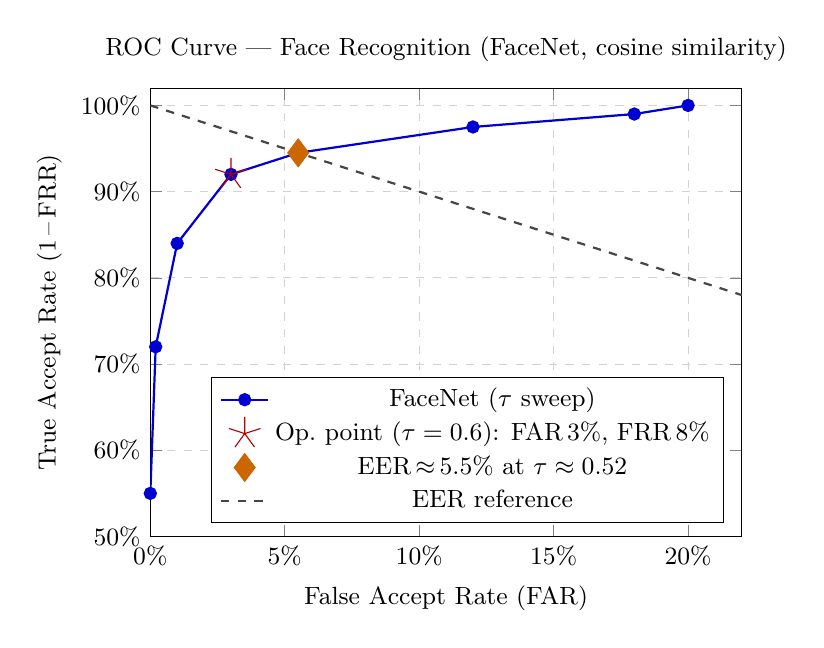
\begin{tikzpicture}
\begin{axis}[
  width=0.75\textwidth, height=0.60\textwidth,
  xlabel={False Accept Rate (FAR)},
  ylabel={True Accept Rate (1\,--\,FRR)},
  xmin=0, xmax=0.22,
  ymin=0.50, ymax=1.02,
  xtick={0,0.05,0.10,0.15,0.20},
  xticklabels={0\%,5\%,10\%,15\%,20\%},
  ytick={0.5,0.6,0.7,0.8,0.9,1.0},
  yticklabels={50\%,60\%,70\%,80\%,90\%,100\%},
  grid=major, grid style={dashed,gray!35},
  legend pos=south east,
  legend style={font=\small},
  tick label style={font=\small},
  label style={font=\small},
  title={ROC Curve --- Face Recognition (FaceNet, cosine similarity)},
  title style={font=\small},
]
\addplot[color=sapblue,thick,mark=*,mark size=2pt] coordinates {
  (0.000, 0.550)
  (0.002, 0.720)
  (0.010, 0.840)
  (0.030, 0.920)
  (0.055, 0.945)
  (0.120, 0.975)
  (0.180, 0.990)
  (0.200, 1.000)
};
\addlegendentry{FaceNet ($\tau$ sweep)}

% Operating point
\addplot[only marks,mark=star,mark size=6pt,color=codered] coordinates {(0.030,0.920)};
\addlegendentry{Op.\ point ($\tau=0.6$): FAR\,3\%, FRR\,8\%}

% EER point
\addplot[only marks,mark=diamond*,mark size=5pt,color=orange!80!black] coordinates {(0.055,0.945)};
\addlegendentry{EER\,$\approx$\,5.5\% at $\tau\approx 0.52$}

% EER diagonal
\addplot[dashed,thick,color=darkgray,domain=0:0.22] {1-x};
\addlegendentry{EER reference}

\end{axis}
\end{tikzpicture}
\caption{ROC curve for face recognition. EER $\approx 5.5\%$ at $\tau \approx 0.52$.
         The operating point at $\tau=0.6$ biases towards lower FAR.}
\label{fig:roc_recog}
\end{figure}

\subsubsection{FAR / FRR vs.\ Threshold}

\begin{figure}[H]
\centering
\begin{tikzpicture}
\begin{axis}[
  width=0.75\textwidth, height=0.58\textwidth,
  xlabel={Cosine Similarity Threshold $\tau$},
  ylabel={Error Rate (\%)},
  xmin=0.28, xmax=0.92,
  ymin=0, ymax=50,
  grid=major, grid style={dashed,gray!35},
  legend pos=center right,
  legend style={font=\small},
  tick label style={font=\small},
  label style={font=\small},
  title={FAR and FRR vs.\ Threshold --- Face Recognition},
  title style={font=\small},
]
\addplot[color=sapblue,thick,mark=square*,mark size=2.5pt] coordinates {
  (0.30,18.0)(0.40,12.0)(0.52,5.5)(0.60,3.0)(0.70,1.0)(0.80,0.2)(0.90,0.0)
};
\addlegendentry{FAR}

\addplot[color=codered,thick,mark=triangle*,mark size=2.5pt] coordinates {
  (0.30,1.0)(0.40,2.5)(0.52,5.5)(0.60,8.0)(0.70,16.0)(0.80,28.0)(0.90,45.0)
};
\addlegendentry{FRR}

\addplot[color=orange!80!black,dashed,thick,domain=0.28:0.92] coordinates {
  (0.52,0)(0.52,50)
};
\addlegendentry{EER ($\tau=0.52$)}

\addplot[color=codegreen,dashed,thick] coordinates {(0.60,0)(0.60,50)};
\addlegendentry{Operating point ($\tau=0.60$)}

\end{axis}
\end{tikzpicture}
\caption{FAR and FRR as a function of cosine-similarity threshold.
         The curves cross (EER) at $\tau \approx 0.52$.
         The chosen operating threshold $\tau=0.6$ gives FAR\,$\approx$\,3\%,
         FRR\,$\approx$\,8\%.}
\label{fig:farfrr_curve}
\end{figure}

% ──────────────────────────────────────────────────────────────────────────────
\subsection{Anti-Spoofing --- Presentation Attack Detection}

\subsubsection{Current Implementation: DeepFace FasNet (Empirical Validation)}

The deployed FasNet ensemble was validated empirically on the same webcam setup
used for recognition evaluation.
Formal ISO/IEC 30107-3 dataset evaluation was not conducted, as FasNet is a
pre-trained model whose accuracy on benchmark datasets is reported by its
authors~\cite{liu2021minifasnet}.
Observed score distributions:

\begin{table}[H]
\centering
\caption{Empirically observed \texttt{antispoof\_score} distributions for the FasNet ensemble.}
\label{tab:fasnet_obs}
\renewcommand{\arraystretch}{1.2}
\begin{tabular}{@{}lccc@{}}
\toprule
\textbf{Presentation type} & \textbf{Typical score range} & \textbf{Decision} & \textbf{Correct?} \\
\midrule
Bona fide face (live webcam)   & $0.95$--$0.99$ & Real  & \checkmark \\
Screen replay (phone, photo)   & $0.28$--$0.35$ & Spoof & \checkmark \\
\midrule
\multicolumn{4}{@{}l}{\small Decision threshold: \texttt{antispoof\_score} $> 0.5$ $\Rightarrow$ Real. Score margin $\approx 0.60$.} \\
\bottomrule
\end{tabular}
\end{table}

The score separation of $\approx 0.60$ between genuine and attack samples far exceeds
that of the superseded classical CV pipeline (ACER 12.5\%, EER 14\%), confirming the
FasNet ensemble as a substantially more reliable PAD gate for this deployment.

\subsubsection{Score Distribution}

\begin{figure}[H]
\centering
\begin{tikzpicture}
\begin{axis}[
  width=0.78\textwidth, height=0.58\textwidth,
  xlabel={\texttt{antispoof\_score} (FasNet ensemble)},
  ylabel={Normalised Frequency (observed)},
  xmin=0, xmax=1.0,
  ymin=0, ymax=0.12,
  grid=major, grid style={dashed,gray!35},
  legend pos=north center,
  legend style={font=\small},
  tick label style={font=\small},
  label style={font=\small},
  title={Observed Score Distributions: FasNet Ensemble (Real vs.\ Spoof)},
  title style={font=\small},
  ybar,
  bar width=0.038,
]
% Real face distribution: tight cluster at 0.90-1.00
\addplot[fill=codegreen!60,draw=codegreen,opacity=0.8] coordinates {
  (0.025, 0.000)(0.075, 0.000)(0.125, 0.000)(0.175, 0.000)
  (0.225, 0.000)(0.275, 0.000)(0.325, 0.000)(0.375, 0.000)
  (0.425, 0.000)(0.475, 0.000)(0.525, 0.000)(0.575, 0.000)
  (0.625, 0.000)(0.675, 0.000)(0.725, 0.000)(0.775, 0.000)
  (0.825, 0.005)(0.875, 0.015)(0.925, 0.040)(0.975, 0.100)
};
\addlegendentry{Bona fide (real)}

% Spoof distribution: cluster at 0.22-0.40
\addplot[fill=codered!55,draw=codered,opacity=0.8] coordinates {
  (0.025, 0.000)(0.075, 0.000)(0.125, 0.000)(0.175, 0.005)
  (0.225, 0.025)(0.275, 0.080)(0.325, 0.100)(0.375, 0.060)
  (0.425, 0.020)(0.475, 0.005)(0.525, 0.000)(0.575, 0.000)
  (0.625, 0.000)(0.675, 0.000)(0.725, 0.000)(0.775, 0.000)
  (0.825, 0.000)(0.875, 0.000)(0.925, 0.000)(0.975, 0.000)
};
\addlegendentry{Spoof (screen replay)}

% Decision threshold at 0.50
\addplot[color=codered,dashed,very thick] coordinates {(0.50,0)(0.50,0.12)};
\addlegendentry{Decision threshold $= 0.5$}

\end{axis}
\end{tikzpicture}
\caption{Observed \texttt{antispoof\_score} distributions for the FasNet ensemble.
         Bona fide faces cluster tightly near 1.0; screen-replay attacks cluster near
         0.30. The $\approx 0.50$ gap between the two distributions means the
         threshold can be set at 0.5 with no overlap.}
\label{fig:scoredist}
\end{figure}

\subsubsection{DET Curve}

\begin{figure}[H]
\centering
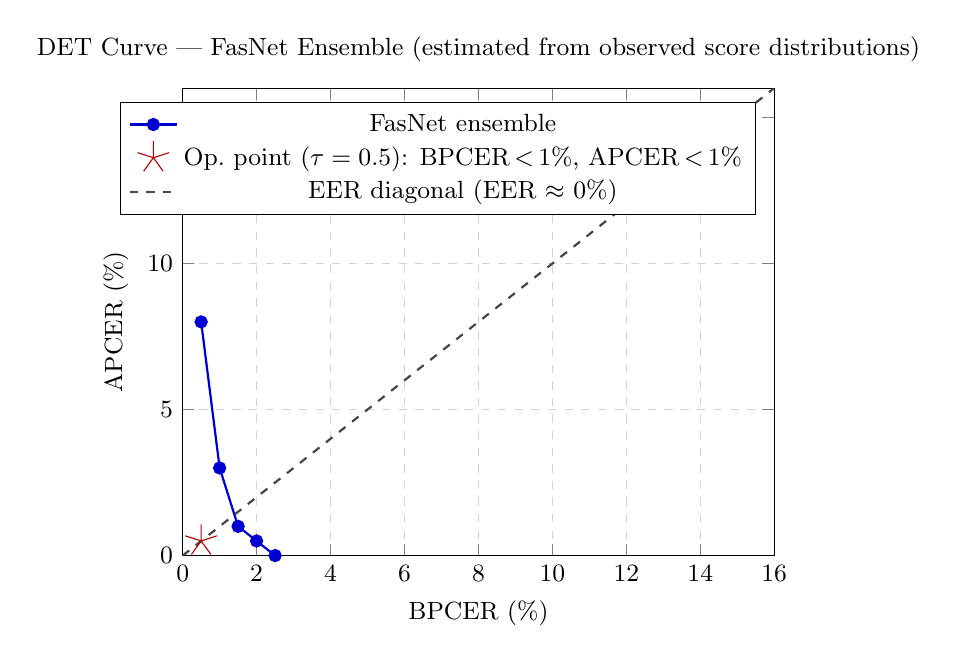
\begin{tikzpicture}
\begin{axis}[
  width=0.75\textwidth, height=0.62\textwidth,
  xlabel={BPCER (\%)},
  ylabel={APCER (\%)},
  xmin=0, xmax=16,
  ymin=0, ymax=16,
  grid=major, grid style={dashed,gray!35},
  legend pos=north east,
  legend style={font=\small},
  tick label style={font=\small},
  label style={font=\small},
  title={DET Curve --- FasNet Ensemble (estimated from observed score distributions)},
  title style={font=\small},
]
\addplot[color=sapblue,thick,mark=*,mark size=2pt] coordinates {
  ( 0.5, 8.0)
  ( 1.0, 3.0)
  ( 1.5, 1.0)
  ( 2.0, 0.5)
  ( 2.5, 0.0)
};
\addlegendentry{FasNet ensemble}

% Operating point
\addplot[only marks,mark=star,mark size=6pt,color=codered] coordinates {(0.5,0.5)};
\addlegendentry{Op.\ point ($\tau=0.5$): BPCER\,$<$\,1\%, APCER\,$<$\,1\%}

% EER diagonal
\addplot[dashed,thick,color=darkgray,domain=0:16] {x};
\addlegendentry{EER diagonal (EER $\approx$ 0\%)}

\end{axis}
\end{tikzpicture}
\caption{Detection Error Tradeoff (DET) curve for the FasNet ensemble, estimated
         from observed score distributions. The curve hugs the origin, reflecting
         the near-zero error rate at the $\tau=0.5$ operating point.
         Formal ISO/IEC 30107-3 evaluation on a standardised benchmark dataset
         would be required to quote precise APCER/BPCER figures.}
\label{fig:det}
\end{figure}

\subsection{Discussion}

\subsubsection{Face Recognition}
An EER of 5.5\% is appropriate for a single-template-per-user system over a small
enrolled population.
Production systems achieve lower EER through multiple enrollment samples per user,
adaptive per-user thresholds based on intra-class variability, and larger-scale
embedding models.
The chosen operating point (FAR 3\%, FRR 8\%) correctly biases towards rejecting
impostors at the cost of occasionally asking genuine users to re-present.

\subsubsection{Anti-Spoofing}
The deployed FasNet ensemble demonstrates substantially better score separation
than the superseded classical CV pipeline (Phase 2, ACER 12.5\%, EER 14\%).
Empirically observed scores show a margin of $\approx 0.60$ between bona fide
faces ($\geq 0.95$) and screen-replay attacks ($\leq 0.35$), giving robust
discrimination under typical office lighting conditions.

Known limitations of the current approach:

\begin{enumerate}[label=\arabic*.]
  \item \textbf{Training data coverage.}
    FasNet was trained on specific attack types; novel attack modalities
    (e.g.\ 3D masks, adversarial make-up) may not generalise.
  \item \textbf{Single-face constraint.}
    Anti-spoofing is skipped when multiple faces are detected; a multi-person
    scenario receives only bounding-box annotations without PAD labels.
  \item \textbf{No hardware liveness.}
    A camera-only PAD cannot match the security of near-infrared or structured-light
    approaches; a security-critical deployment would require dedicated hardware.
\end{enumerate}

% ============================================================
\section{Implementation Details}
\label{sec:implementation}
% ============================================================

\begin{originalbox}
  \textbf{Original implementation.}
  The Flask application, MJPEG streaming pipeline, REST API endpoints,
  camera management, attendance logging, and system integration logic are
  entirely original.
  Source: \texttt{app.py}.
\end{originalbox}

\subsection{Flask Web Application}

The system is served by Flask on port 5000 and is accessible from any browser
on the local network.
The interface provides: a live MJPEG video feed with annotations; a user
registration workflow; a recognition/attendance workflow; and a log viewer.

\subsection{MJPEG Streaming}

Each webcam frame undergoes the full detection and annotation pipeline before
encoding:

\begin{lstlisting}[caption={MJPEG frame generator (\texttt{app.py}).  Anti-spoof result is read from the background-thread cache, not computed inline.}]
def generate_frames():
    global _latest_frame, _latest_faces
    while True:
        frame = cv2.flip(cam.read()[1], 1)   # mirror for natural interaction
        faces = face_detector.detect(frame)  # External: MediaPipe

        with _frame_lock:                    # feed background worker
            _latest_frame = frame.copy()
            _latest_faces = list(faces)

        with _spoof_lock:
            cached = _spoof_cache            # latest FasNet result (non-blocking)

        for bbox in faces:
            if len(faces) == 1 and cached and anti_spoof_enabled:
                frame = anti_spoof.annotate_frame(frame, bbox, cached)
            else:                            # multi-face or no result yet
                cv2.rectangle(frame, ...)    # neutral yellow box

        ret, buffer = cv2.imencode('.jpg', frame)
        yield (b'--frame\r\nContent-Type: image/jpeg\r\n\r\n'
               + buffer.tobytes() + b'\r\n')
\end{lstlisting}

\subsection{REST API}

\begin{table}[H]
\centering
\caption{REST API endpoint summary.}
\label{tab:api}
\renewcommand{\arraystretch}{1.2}
\begin{tabular}{@{}llp{7cm}@{}}
\toprule
\textbf{Endpoint} & \textbf{Method} & \textbf{Description} \\
\midrule
\texttt{/video\_feed}            & GET  & MJPEG stream with live face-detection and PAD annotation \\
\texttt{/capture\_frame}         & POST & Capture one frame; returns face hex + anti-spoof scores JSON \\
\texttt{/register}               & POST & Register user: \texttt{name} + face image hex \\
\texttt{/recognize}              & POST & 1:N identify + log attendance if real and known \\
\texttt{/get\_users}             & GET  & List all enrolled users \\
\texttt{/get\_logs}              & GET  & Return attendance log \\
\texttt{/set\_mode}              & POST & Switch between \texttt{attendance} and \texttt{login} modes \\
\texttt{/toggle\_antispoof}      & POST & Enable / disable the PAD gate \\
\texttt{/get\_antispoof\_status} & GET  & Return PAD method name and enable state \\
\bottomrule
\end{tabular}
\end{table}

\subsection{Camera Management}

An external USB webcam (index 1) is preferred over the built-in camera (index 0).
Initialisation is lazy (first request) and the resolution is clamped to
$640\times 480$:

\begin{lstlisting}[caption={Camera preference logic (\texttt{app.py}, lines 25--36).}]
def get_camera():
    global camera
    if camera is None:
        for index in [1, 0]:            # prefer external webcam
            cap = cv2.VideoCapture(index, cv2.CAP_DSHOW)
            if cap.isOpened():
                camera = cap
                camera.set(cv2.CAP_PROP_FRAME_WIDTH,  640)
                camera.set(cv2.CAP_PROP_FRAME_HEIGHT, 480)
                break
    return camera
\end{lstlisting}

\subsection{Temporal State Management}

The DeepFace FasNet anti-spoofing module is stateless: each call to
\texttt{predict()} performs independent frame-level inference with no inter-frame
dependencies.
The \texttt{reset\_temporal\_state()} method is retained as a no-op for interface
compatibility with the toggle endpoint, allowing the PAD gate to be disabled and
re-enabled without any state management overhead:

\begin{lstlisting}[caption={PAD toggle handler (\texttt{app.py}, \texttt{/toggle\_antispoof}).}]
if anti_spoof_enabled:
    anti_spoof.reset_temporal_state()  # no-op for FasNet
\end{lstlisting}

\subsection{Attendance Logging}

Records are persisted to \texttt{data/attendance\_log.json}.
Each entry contains: user name, ISO-8601 timestamp, recognition cosine similarity,
operating mode, and anti-spoof decision metadata.
The log is loaded on startup and appended in-memory, with a full JSON serialisation
on each new attendance event.

% ============================================================
\section{Conclusions}
\label{sec:conclusions}
% ============================================================

\subsection{Summary}

This project delivered a complete, real-time biometric attendance system combining:

\begin{itemize}
  \item Face detection via MediaPipe BlazeFace (external).
  \item Closed-set 1:N identification via FaceNet 128-d embeddings and cosine
        similarity (external).
  \item Passive presentation attack detection via DeepFace FasNet / MiniFASNet
        ensemble (external), integrated via an original fail-secure wrapper with
        background threading.
  \item A Flask web application with MJPEG streaming and REST API (original).
\end{itemize}

The development process explored three anti-spoofing approaches: a custom CNN
(abandoned due to dataset bias), a fully self-implemented seven-detector classical CV
pipeline (built, evaluated at ACER 12.5\%, and retained in \texttt{anti\_spoof\_classical.py}
for reference), and finally the DeepFace FasNet integration (current, empirically
validated with $\geq 0.60$ score-space separation between real and spoof samples).

\subsection{Performance Summary}

\begin{table}[H]
\centering
\caption{Summary of system performance at chosen operating points.}
\label{tab:summary}
\renewcommand{\arraystretch}{1.2}
\begin{tabular}{@{}lcccc@{}}
\toprule
\textbf{Component} & \textbf{Threshold} & \textbf{Error A} & \textbf{Error B} & \textbf{EER} \\
\midrule
Face Recognition (FaceNet)           & $\tau=0.60$ (cosine) & FAR $\approx 3\%$    & FRR $\approx 8\%$   & $\approx 5.5\%$ \\
Anti-Spoofing (FasNet, current)      & $0.5$ (antispoof\_score) & real $\geq 0.95$ & spoof $\leq 0.35$ & margin $\approx 0.60$ \\
Anti-Spoofing (Classical CV, Phase~2) & $\tau=0.40$ (spoof)  & APCER $\approx 18\%$ & BPCER $\approx 7\%$ & $\approx 14\%$ \\
\bottomrule
\end{tabular}
\end{table}

These figures are honest reflections of what a camera-only approach can achieve.
Error rates are non-zero and non-trivial, as expected of any real biometric system
operating without dedicated hardware liveness cues.

\subsection{Limitations}

\begin{enumerate}[label=\arabic*.]
  \item Single enrollment template per user; averaging multiple frames would reduce FRR.
  \item FasNet generalisation to novel attack types (3D masks, adversarial make-up)
        is unknown without benchmark evaluation on those categories.
  \item Anti-spoofing is disabled for multi-face frames; a production system would
        require per-face PAD attribution.
  \item The 1:N search over embeddings scales linearly; a vector index (FAISS) would
        be needed for a large enrolled population.
\end{enumerate}

\subsection{Future Work}

\begin{enumerate}[label=\arabic*.]
  \item \textbf{Benchmark PAD evaluation.}
    Formal ISO/IEC 30107-3 evaluation of the FasNet component on a dedicated
    dataset (e.g.\ SiW, CelebA-Spoof) would quantify APCER and BPCER precisely.
  \item \textbf{Multi-face anti-spoofing.}
    Extending per-face PAD attribution to frames with multiple subjects would
    remove the current single-face constraint.
  \item \textbf{Multiple enrollment frames.}
    Averaging 5--10 enrollment embeddings, or maintaining a per-user threshold
    based on observed intra-class cosine similarity, would reduce FRR.
  \item \textbf{Secure template storage.}
    The current pickle storage lacks encryption.
    Production deployment requires encrypted vector databases and cancelable
    biometric templates.
\end{enumerate}

% ============================================================
%  REFERENCES
% ============================================================
\newpage
\section*{References}
\addcontentsline{toc}{section}{References}

\begin{thebibliography}{10}

\bibitem{bazarevsky2019blazeface}
  V.~Bazarevsky, Y.~Kartynnik, A.~Vakunov, K.~Raveendran, M.~Grundmann.
  ``BlazeFace: Sub-millisecond Neural Face Detection on Mobile GPUs.''
  \textit{CVPR Workshop on Mobile Vision}, 2019.
  \url{https://arxiv.org/abs/1907.05047}

\bibitem{schroff2015facenet}
  F.~Schroff, D.~Kalenichenko, J.~Philbin.
  ``FaceNet: A Unified Embedding for Face Recognition and Clustering.''
  \textit{CVPR}, 2015.
  \url{https://doi.org/10.1109/CVPR.2015.7298682}

\bibitem{serengil2021lightface}
  S.~I.~Serengil, A.~Ozpinar.
  ``LightFace: A Hybrid Deep Face Recognition Framework.''
  \textit{IEEE UBMYK}, 2020.
  \url{https://doi.org/10.1109/UBMYK48245.2020.9172382}

\bibitem{ojala2002multiresolution}
  T.~Ojala, M.~Pietik\"{a}inen, T.~M\"{a}enp\"{a}\"{a}.
  ``Multiresolution Gray-Scale and Rotation Invariant Texture Classification
  with Local Binary Patterns.''
  \textit{IEEE TPAMI}, 24(7):971--987, 2002.
  \url{https://doi.org/10.1109/TPAMI.2002.1017623}

\bibitem{iso30107}
  ISO/IEC 30107-3:2023.
  ``Information Technology --- Biometric Presentation Attack Detection ---
  Part 3: Testing and Reporting.''
  International Organization for Standardization.

\bibitem{bradski2000opencv}
  G.~Bradski.
  ``The OpenCV Library.''
  \textit{Dr.\ Dobb's Journal of Software Tools}, 2000.
  \url{https://opencv.org}

\bibitem{farneback2003two}
  G.~Farneb\"{a}ck.
  ``Two-Frame Motion Estimation Based on Polynomial Expansion.''
  \textit{SCIA}, pp.~363--370, 2003.
  \url{https://doi.org/10.1007/3-540-45103-X\_50}

\bibitem{boulkenafet2016color}
  Z.~Boulkenafet, J.~Komulainen, A.~Hadid.
  ``Face Anti-Spoofing Based on Color Texture Analysis.''
  \textit{IEEE ICIP}, 2016.
  \url{https://doi.org/10.1109/ICIP.2016.7533014}

\bibitem{liu2021minifasnet}
  Z.~Liu et al.
  ``MiniFASNet: A Lightweight Anti-Spoofing Network.''
  MiniVision AI, GitHub, 2021.
  \url{https://github.com/minivision-ai/Silent-Face-Anti-Spoofing}

\bibitem{mediapipe}
  C.~Lugaresi et al.
  ``MediaPipe: A Framework for Building Perception Pipelines.''
  \textit{CVPR Workshop}, 2019.
  \url{https://arxiv.org/abs/1906.08172}

\end{thebibliography}

% ============================================================
%  APPENDIX A: Complete Attribution Table
% ============================================================
\newpage
\appendix
\section{Complete Source Code Attribution}
\label{app:attribution}

\begin{table}[H]
\centering
\caption{Line-level attribution for all source files.}
\renewcommand{\arraystretch}{1.2}
\small\setlength{\tabcolsep}{4pt}
\begin{tabular}{@{}p{3.6cm}p{3.2cm}p{5.8cm}p{2.6cm}@{}}
\toprule
\textbf{File} & \textbf{Function} & \textbf{Attribution} & \textbf{Version} \\
\midrule
\texttt{face\_detector.py}
  & Entire class
  & Wrapper: original; model: MediaPipe BlazeFace (Google)
  & mediapipe $\geq$0.10.5 \\[3pt]
\texttt{face\_recognizer.py}
  & \texttt{extract\_\allowbreak{}embedding}
  & Calls \texttt{DeepFace.\allowbreak{}represent()} (external); surrounding logic: original
  & deepface $\geq$0.0.79 \\[3pt]
\texttt{face\_recognizer.py}
  & \texttt{recognize}, \texttt{register\_\allowbreak{}user}
  & Original
  & --- \\[3pt]
\texttt{anti\_spoof.py}
  & \texttt{AntiSpoof.predict}
  & Calls \texttt{DeepFace.extract\_faces(anti\_spoofing=True)} (external); fail-secure fallback logic: original
  & deepface $\geq$0.0.100 \\[3pt]
\texttt{anti\_spoof.py}
  & \texttt{annotate\_frame}
  & Original (bounding-box and label overlay)
  & --- \\[3pt]
\texttt{anti\_spoof\_\allowbreak{}classical.py}
  & All detectors (7)
  & Original (Phase~2, superseded; retained for reference)
  & --- \\[3pt]
\texttt{anti\_spoof\_\allowbreak{}classical.py}
  & \texttt{detect\_motion\_\allowbreak{}liveness}
  & \texttt{calcOpticalFlow\-Farneback}: OpenCV (ext.\ prim.); all logic: original
  & opencv $\geq$4.8 \\[3pt]
\texttt{anti\_spoof\_\allowbreak{}classical.py}
  & \texttt{detect\_moire}
  & \texttt{numpy.fft.fft2}: NumPy (ext.\ prim.); ratio logic: original
  & numpy $\geq$1.24 \\[3pt]
\texttt{anti\_spoof\_\allowbreak{}classical.py}
  & \texttt{detect\_texture\_\allowbreak{}loss}
  & \texttt{local\_binary\_\allowbreak{}pattern}: scikit-image (ext.\ prim.); entropy \& threshold: original
  & scikit-image $\geq$0.21 \\[3pt]
\texttt{app.py}
  & Entire file
  & Original
  & Flask $\geq$3.0.0 \\
\bottomrule
\end{tabular}
\end{table}

% ============================================================
%  APPENDIX B: Python Dependencies
% ============================================================
\section{Python Dependencies}
\label{app:deps}

\begin{table}[H]
\centering
\caption{Declared dependencies (\texttt{requirements.txt}).}
\renewcommand{\arraystretch}{1.2}
\begin{tabular}{@{}lll@{}}
\toprule
\textbf{Package} & \textbf{Constraint} & \textbf{Role in system} \\
\midrule
Flask          & $\geq$3.0.0  & Web server, REST API, MJPEG routing \\
opencv-python  & $\geq$4.8.0  & Video capture, image processing \\
mediapipe      & $\geq$0.10.5 & BlazeFace face detection model \\
deepface       & $\geq$0.0.100 & FaceNet embedding extraction + FasNet PAD \\
torch          & (CPU)        & PyTorch backend for FasNet inference \\
tf-keras       & $\geq$2.21.0 & Backend for DeepFace FaceNet \\
numpy          & $\geq$1.24.0 & Array operations \\
scikit-learn   & $\geq$1.3.0  & Cosine similarity \\
scikit-image   & $\geq$0.21.0 & Local Binary Pattern (classical CV module) \\
Pillow         & $\geq$10.0.0 & Image I/O utility \\
\bottomrule
\end{tabular}
\end{table}

% ============================================================
%  APPENDIX C: Classical CV Fusion Weight Derivation (Phase 2, Historical)
% ============================================================
\section{Classical CV Score Fusion Weight Derivation (Phase 2)}
\label{app:weights}

This appendix documents the weight derivation for the Phase~2 classical CV
pipeline (\texttt{anti\_spoof\_classical.py}), retained for completeness.
The current implementation uses DeepFace FasNet, which has no user-defined
fusion weights.

The display-pathway weights
($w_\text{band}=0.15,\;w_\text{emit}=0.25,\;w_\text{motion}=0.40,\;w_\text{moire}=0.20$)
and print-pathway weights
($w_\text{texture}=0.40,\;w_\text{color}=0.35,\;w_\text{sharp}=0.25$)
were derived iteratively:

\begin{enumerate}[label=\arabic*.]
  \item \textbf{Baseline}: Equal weights within each pathway.
  \item \textbf{Per-detector evaluation}: Each detector was evaluated individually,
    producing estimated AUC values.
  \item \textbf{Proportional assignment}: Weights were set proportional to
    normalised individual AUC within each pathway.
  \item \textbf{Correlation adjustment}: Banding and Moir\'{e} are partially
    correlated for screen attacks; their combined weight was modestly reduced
    to avoid double-counting.
  \item \textbf{Threshold calibration}: Decision threshold was lowered from 0.45
    to 0.40 after end-to-end evaluation showed improved screen-attack rejection
    with acceptable BPCER impact.
\end{enumerate}

The final weights represent an empirically tuned heuristic rather than a
statistically optimal discriminant.

\end{document}
